\chapter{System Models}

\section{Scenarios}
The scenarios are based on Node.js based web applications on a server running root and rootJS\\

Web viewer launches and provides a GUI to its end user	\\
Web viewer requests data for visualization by calling rootJS\\
\indent	Node.js invokes ROOT I/O operations\\
\indent \indent		ROOT loads data and provides raw visualization data\\
\indent	Node.js serializes data and streams it to the web viewer\\
Web viewer receives data and renders it in the browser\\
\section{Use Cases}

\pagebreak[4]

\section{Object Models}
Figure 6.1 illustrates what the bindings architecture may look like.
\textit{RootApplication::init} exposes the available variables, functions and classes via V8 to JavaScript.
Exposed functions call \textit{methodProxy}, which uses the callee function name to determine the ROOT function that should be called. This will also handle callbacks which are passed via the \textit{args} parameter.
The \textit{classProxy} is called instead of \textit{methodProxy} when the specified function is a constructor. This will use \textit{ProxyObjectFactory} to generate a JavaScript object.
The \textit{globalGetter} and \textit{globalSetter} method are called when a global variable should be accessed. Again the \textit{ProxyObjectFactory} will be used in this case to generate corresponding JavaScript objects.
\\\\
The \textit{ProxyObjectFactory} creates an instance of a subclass of \textit{ProxyObject}, the acutal subclass will be decided by using the \textit{type} parameter.
If the \textit{ProxyObject} contains a scalar type (like int, long, string, ...) the \textit{getV8Handle} method will simply return the corresponding V8 handle with the value at the defined address.
If the \textit{ProxyObject} contains an object, \textit{getV8Handle} will recursively call the \textit{ProxyObjectFactory} for every element it contains and builds a JavaScript object.
To handle reference circles we use a caching mechanism that stores already created \textit{v8::handle}s to reuse them.

\begin{figure}[htb]
	\centering
	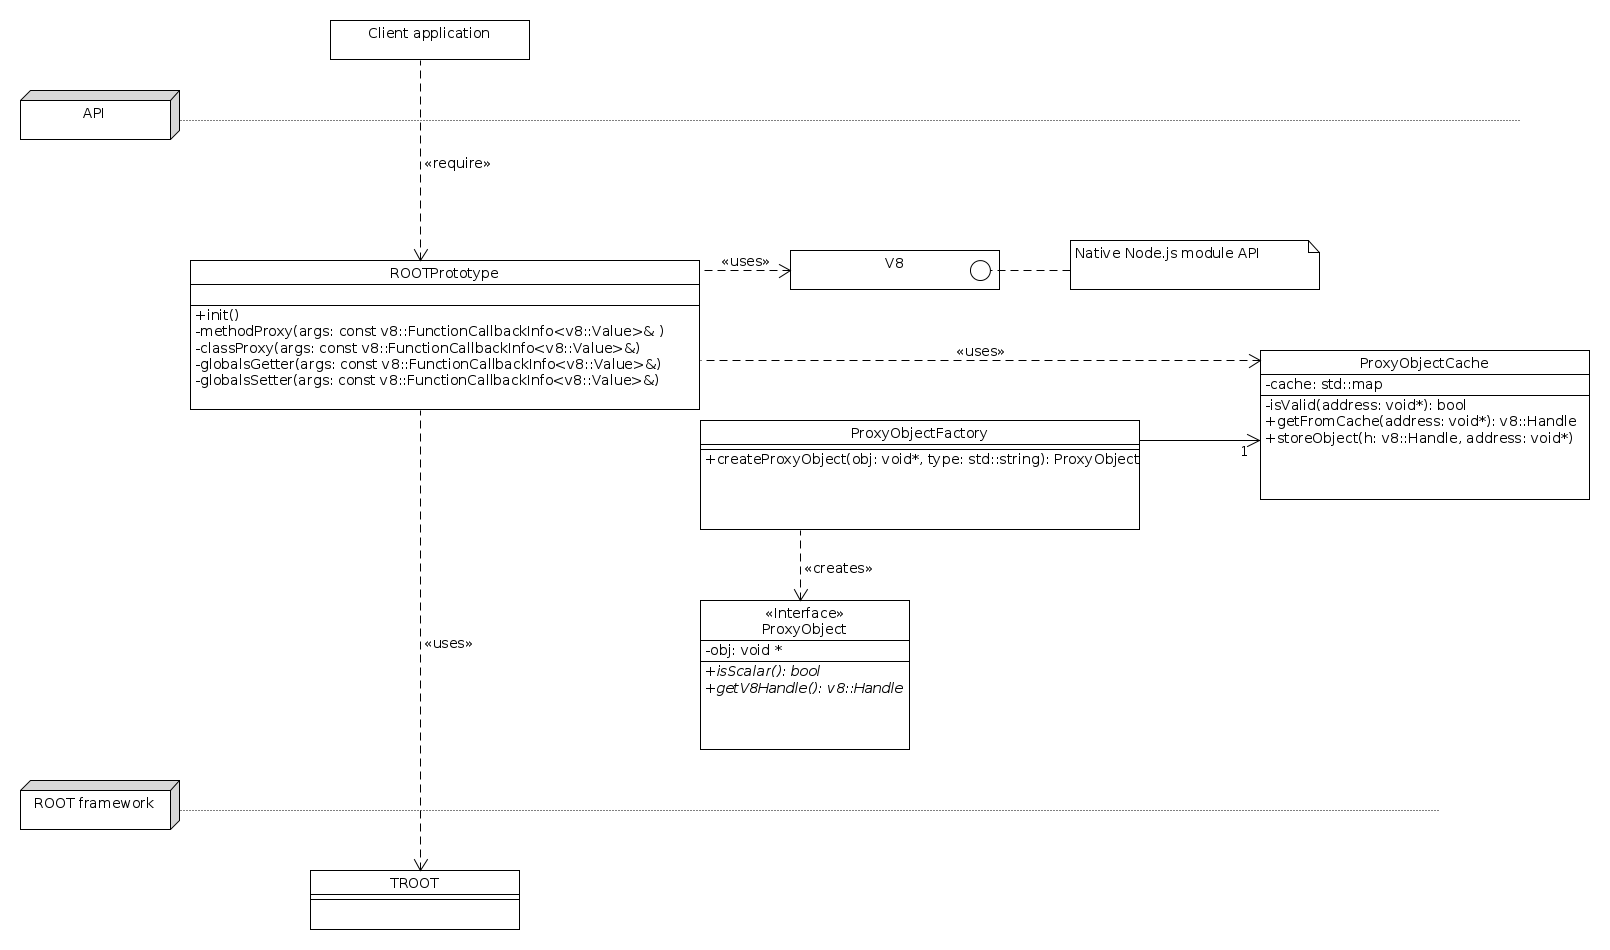
\includegraphics[width=18cm]{./latex/resources/architecture.png}
	\caption{basic architecture draft}
\end{figure}

\pagebreak[4]

\section{Dynamic Models}
The following figure shows how rootJS initializes upon being called the first time by a client application. As bindings do not add any functionality of their own, the client application is not further specified. After the bindings are initialized the client application may use any root functionality through the roootJS API.
\begin{figure}[htb]
	\centering
	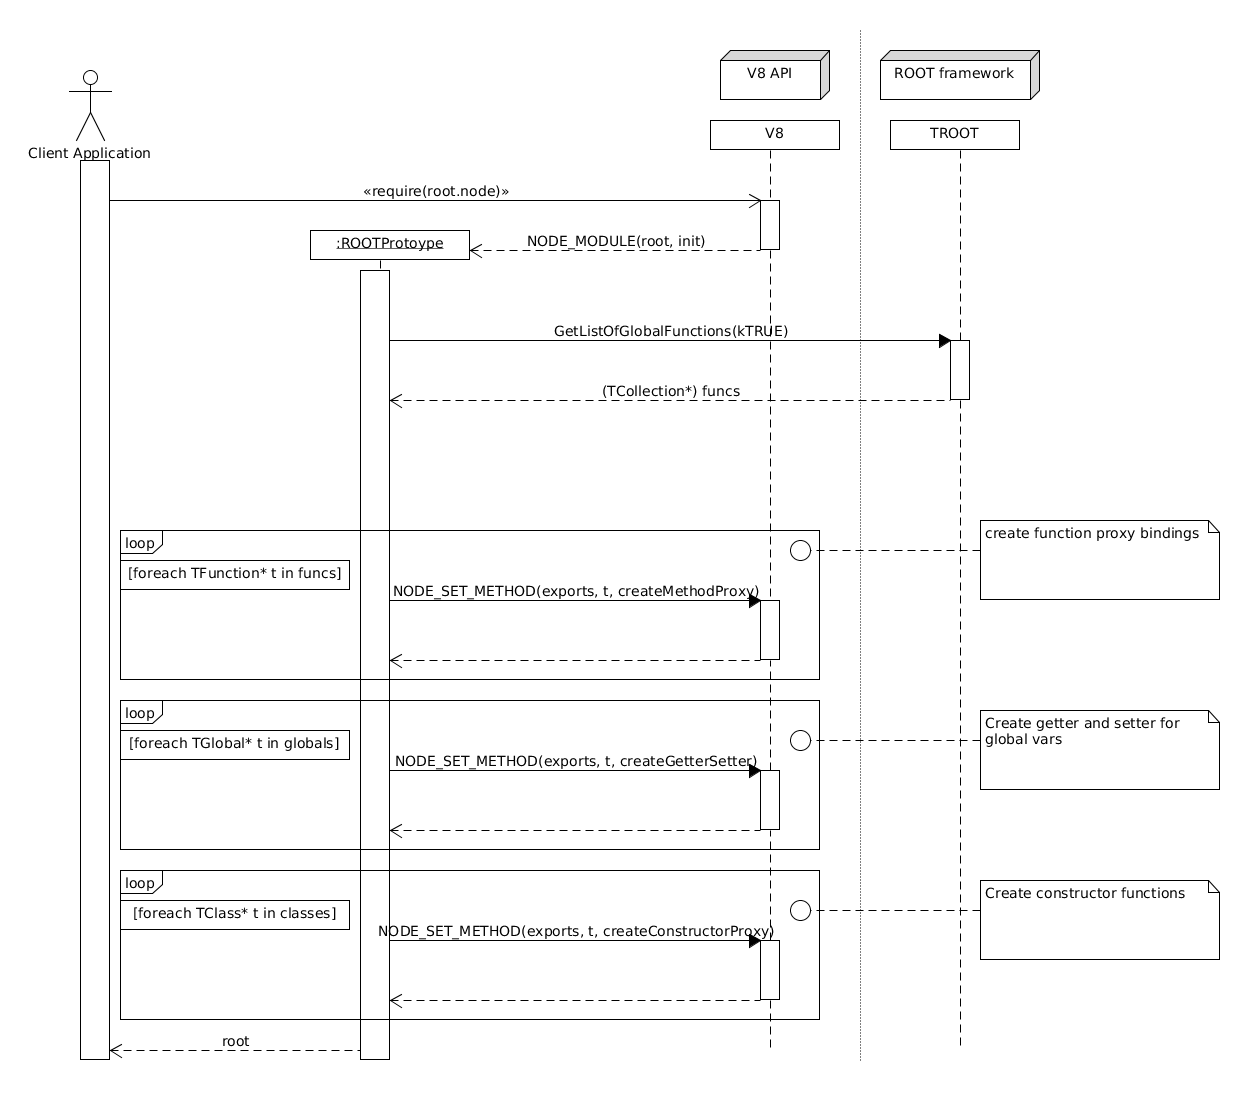
\includegraphics[width=18cm]{./latex/resources/startupSequence.png}
	\caption{startup sequence}
\end{figure}
